\def\mytitle{MATRICES USING PYTHON}
\def\myauthor{V.GOKULKUMAR}
\def\contact{velicharlagokulkumar@gmail.com}
\def\mymodule{Future Wireless Communication (FWC)}
\documentclass[10pt, a4paper]{article}
\usepackage[a4paper,outer=1.5cm,inner=1.5cm,top=1.75cm,bottom=1.5cm]{geometry}
\twocolumn
\usepackage{graphicx}
\graphicspath{{./images/}}
\usepackage[colorlinks,linkcolor={black},citecolor={blue!80!black},urlcolor={blue!80!black}]{hyperref}
\usepackage[parfill]{parskip}
\usepackage{lmodern}
\usepackage{tikz}
	\usepackage{physics}
%\documentclass[tikz, border=2mm]{standalone}
%\usepackage{karnaugh-map}
%\documentclass{article}
\usepackage{tabularx}
%\usepackage{circuitikz}
\usepackage{enumitem}
\usetikzlibrary{calc}
\usepackage{amsmath}
\usepackage{amssymb}
\renewcommand*\familydefault{\sfdefault}
\usepackage{watermark}
\usepackage{lipsum}
\usepackage{xcolor}
\usepackage{listings}
\usepackage{float}
\usepackage{titlesec}
\providecommand{\mtx}[1]{\mathbf{#1}}
\titlespacing{\subsection}{1pt}{\parskip}{3pt}
\titlespacing{\subsubsection}{0pt}{\parskip}{-\parskip}
\titlespacing{\paragraph}{0pt}{\parskip}{\parskip}
\newcommand{\figuremacro}[5]{
    \begin{figure}[#1]
        \centering
        \includegraphics[width=#5\columnwidth]{#2}
        \caption[#3]{\textbf{#3}#4}
        \label{fig:#2}
    \end{figure}
}

\newcommand{\myvec}[1]{\ensuremath{\begin{pmatrix}#1\end{pmatrix}}}
\let\vec\mathbf
\lstset{
frame=single, 
breaklines=true,
columns=fullflexible
}
\thiswatermark{\centering \put(181,-119.0){
\includegraphics[scale=0.13]{iith_logo3}} }
\title{\mytitle}
\author{\myauthor\hspace{1em}\\\contact\\FWC22034\hspace{6.5em}IITH\hspace{0.5em}\mymodule\hspace{6em}Assignment}
\begin{document}
	\maketitle
	\tableofcontents
   \section{Problem}
  Let A be the centre of the circle $x^2 + y^2-2x-4y-20=0$. Suppose the tangents at the points  B(1,7) and D(4.-2) on the circle meet at the point C. Find the area of the quadrilateral ABCD.
\section{Construction}
  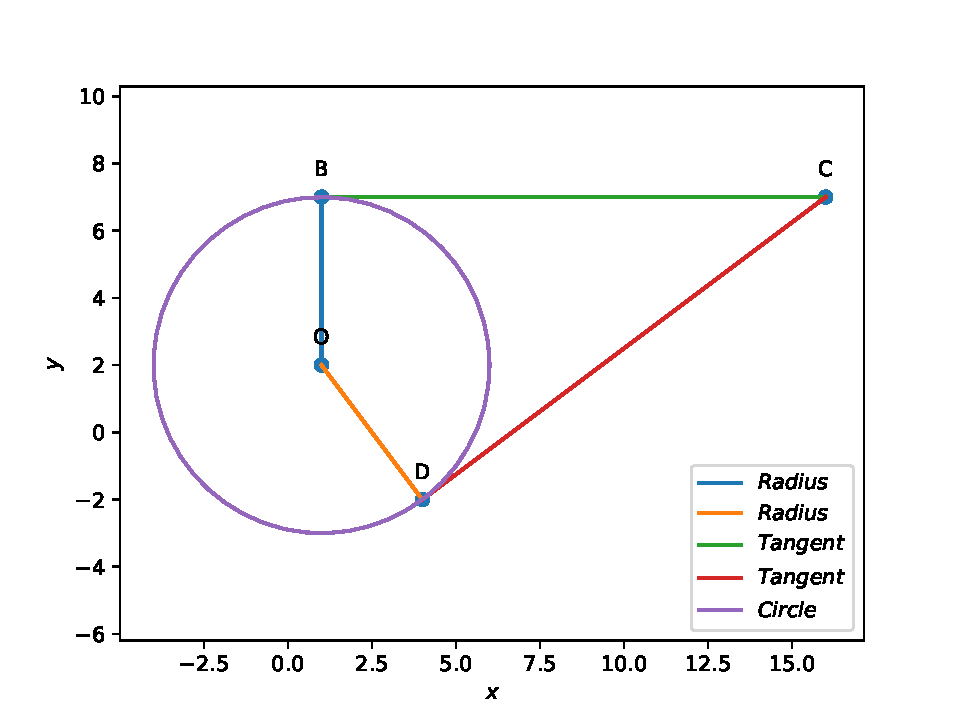
\includegraphics[scale=0.47]{matrix.pdf}
  	\begin{center}
  Figure of construction
  	\end{center}
  \section{Solution}

Circle equation : $x^2+y^2-2x-4y-20=0$\\
The standard equation of the conics is given as :
\begin{align}
\vec{x}^{\top}\vec{V}\vec{x}+2\vec{u}^{\top}\vec{x}+f=0
\end{align}
The given circle  can be expressed as conics with \\parameters
\begin{align}
	\vec{V} &= \vec{I}, \vec{u} = -\myvec{1 \\2}, f = -20
	\end{align}
	Radius and Centre are
	\begin{align}
	r &=\sqrt{{\vec{u}^{\top}\vec{u}}-f },\vec{A}=-u
    \end{align}
    The steps for constructing above figure are :
\begin{enumerate}
 \item Generate a circle of radius $r$ with centre $\vec{A}$ 
 \item Locate $\vec{B}$,$\vec{D}$ on the circle
 \item Find the Normal vectors to $\vec{A}$$\vec{B}$,$\vec{A}$$\vec{D}$ say $\vec{m}_1$,$\vec{m}_2$
\item Find the equations of the tangents and use them to find the intersection $\vec{C}$
\end{enumerate}
    The input parameters for this construction are
\begin{center}
\begin{tabular}{|c|c|c|}
	\hline
	\textbf{Symbol}&\textbf{Value}&\textbf{Description}\\
	\hline
	$\vec{A}$ &\myvec{1\\2}& Centre\\
	\hline
    $\vec{B}$ &\myvec{1\\7}&Point B\\
	\hline
 $\vec{D}$&\myvec{4\\-2}&Point D\\
	\hline
\end{tabular}
\end{center}
$\vec{C}$ is obtained as the point of intersection of the tangents at $\vec{B}$ and $\vec{D}$ 
The equation of both tangents are respectively 
\begin{align}
	\begin{split}
	\vec{x} &= \vec{B} + \lambda_1 \vec{m}_1
\\
		\vec{x} &= \vec{D} + \lambda_2 \vec{m}_2
		\label{eq:quad-circ-lam-B}
	\end{split}
\end{align}
and their intersection is given by 
\begin{align}
	 \vec{B} + \lambda_1 \vec{m}_1
	&	= \vec{D} + \lambda_2 \vec{m}_2
	\\
	\implies \myvec{\vec{m}_1 & \vec{m}_2}\myvec{\lambda_1 \\ -\lambda_2 } &= \vec{D}-\vec{B}
\end{align}
which can be used to obtained $\lambda_1, \lambda_2$ and consequently $\vec{C}$, using 
		\eqref{eq:quad-circ-lam-B}
		\begin{center}
		$\therefore$ Coordinates of C is  $\vec{C} = \myvec{16 \\ 7}$\\
		\end{center}
Letting,
\begin{align}
\vec{v1}=\vec{A}-\vec{B}\\
\vec{v2}=\vec{A}-\vec{C}
\end{align}		
	Area of the $\Delta$ABC is given by 
	\begin{align}
&=\frac{1}{2}\norm{\vec{v1}\times\vec{v2}}
\end{align}
	Area of the of quadrilateral ABCD is given by 
	\begin{align}
&=2\times\frac{1}{2}\norm{\vec{v1}\times\vec{v2}}
\end{align}
$\therefore$The area of quadrilateral ABCD=75 sq.units\\
\textbf{termux commands :}
\begin{lstlisting}
bash sh2.sh............using shell command
\end{lstlisting}
\begin{center}
Below python code realizes the above construction :
\fbox{\parbox{8.5cm}{\url{https://github.com/velicharlagokulkumar/FWC_module1/blob/main/matrices/circle/codes/matrix.py}}}
\end{center}
\end{document}
ent}